\documentclass{article}
\usepackage{amsmath,amssymb,amsfonts}
\usepackage{xcolor}
\usepackage{tikz}
\usetikzlibrary{positioning, calc}

\begin{document}

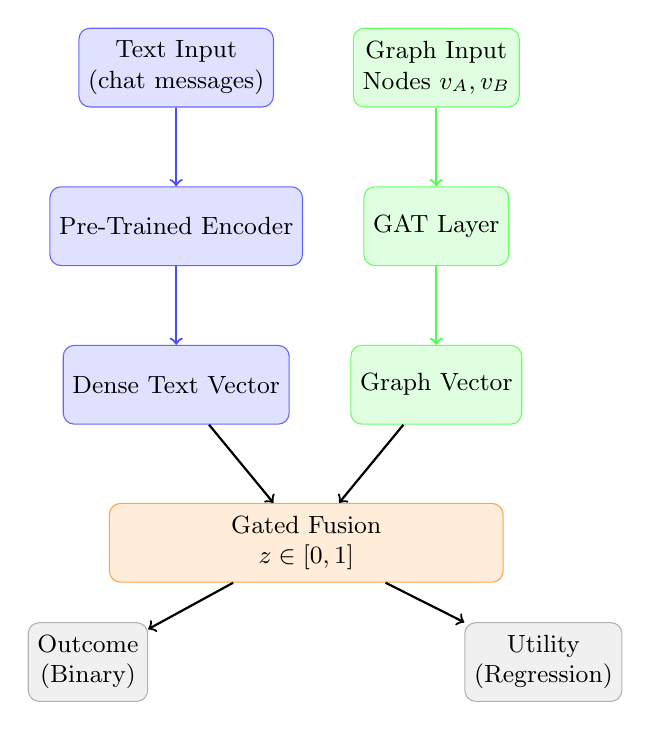
\begin{tikzpicture}[
    node distance=1 cm and 1 cm,
    every node/.style={
        draw,
        rounded corners,
        align=center,
        minimum height=1cm,
        font=\small
    },
    textnode/.style={fill=blue!12, draw=blue!60},
    graphnode/.style={fill=green!12, draw=green!60},
    fusionnode/.style={fill=orange!15, draw=orange!70, minimum width=5cm},
    outnode/.style={fill=gray!12, draw=gray!60},
    arrow/.style={->, thick}
]
% (Your original TikZ code remains exactly as provided)
\node[textnode] (text_input) {Text Input\\(chat messages)};
\node[textnode] (roberta) [below=of text_input] {Pre-Trained Encoder};
\node[textnode] (text_vec) [below=of roberta] {Dense Text Vector};
\node[graphnode] (graph_input) [right=1 cm of text_input] {Graph Input\\Nodes $v_A, v_B$};
\node[graphnode] (gat) [below=of graph_input] {GAT Layer};
\node[graphnode] (graph_vec) [below=of gat] {Graph Vector};
\node[fusionnode] (fusion) [below=1.5 cm of $(text_vec)!0.5!(graph_vec)$] {Gated Fusion\\$z \in [0,1]$};
\node[outnode] (outcome) [below left=.5 cm and -.5 cm of fusion] {Outcome\\(Binary)};
\node[outnode] (utility) [below right=.5 cm and -0.5 cm of fusion] {Utility\\(Regression)};
\draw[arrow, blue!70] (text_input) -- (roberta);
\draw[arrow, blue!70] (roberta) -- (text_vec);
\draw[arrow] (text_vec) -- (fusion);
\draw[arrow, green!70] (graph_input) -- (gat);
\draw[arrow, green!70] (gat) -- (graph_vec);
\draw[arrow] (graph_vec) -- (fusion);
\draw[arrow] (fusion) -- (outcome);
\draw[arrow] (fusion) -- (utility);
\end{tikzpicture}

\end{document}